
\documentclass[11pt]{article}
\usepackage[utf8]{inputenc}
\usepackage[]{hyperref}  
\usepackage[]{listings}
\usepackage[ngerman]{babel}
\usepackage[T1]{fontenc}
\usepackage{graphicx}
\usepackage{minted}
\usepackage{lmodern}
\usepackage[activate={true,nocompatibility},final,tracking=true,kerning=true,spacing=true,factor=1100,stretch=10,shrink=10]{microtype}
\lstset{literate=%
	{Ö}{{\"O}}1
	{Ä}{{\"A}}1
	{Ü}{{\"U}}1
	{ß}{{\ss}}1
	{ü}{{\"u}}1
	{ä}{{\"a}}1
	{ö}{{\"o}}1
}
\fboxsep1px

\setminted[bash]{fontsize=\small,tabsize=2,breaklines,style=bw}

% TODO UPDATE PICS with olat
\begin{document}
 \pagenumbering{gobble}
 \hypersetup{pageanchor=false}
\begin{titlepage}
	\begin{center}
		
		\vspace{6cm}
		
		{\huge Nutzerdokumentation SQLChecker 1.2.0}
		{\small Version Sommersemester 2020}
		\vspace{0.2cm}
		
		
		
		\vspace{2cm}
		
\includegraphics[width=6cm]{figures/goethe}
		\vspace{2.5cm}
		
		Databases and Information Systems (DBIS)
		
		Johann Wolfgang Goethe-Universität Frankfurt am Main
		
		
	\end{center}
	\vspace*{\fill}
	%{\small Version \texttt{1.0}}
	
\end{titlepage}
 \hypersetup{pageanchor=true}
 
\pagenumbering{arabic}
\tableofcontents
 \newpage
\section{Übersicht}
Der \textit{SQLChecker} ist ein Open-Source-Java-Programm, entwickelt als Unterstützung für die Datenbanken-Vorlesung der Goethe Universität Frankfurt am Main.
Die Anwendung ermöglicht Studenten das Erstellen und Testen von SQL-Queries für vorgegebene Aufgaben. Mit Hilfe des Programms können die Statements einfach automatisiert getestet und ausgewertet werden.
Für die Verbindung mit der Datenbank ist \textit{MariaDB} empfohlen.
Das Projekt wird auf GitHub  \href{https://github.com/ptrckbnck/SQLChecker}{\texttt{https://github.com/ptrckbnck/SQLChecker}} zur Verfügung gestellt.

\section{Quickstart}
\subsection{Installation}
\begin{itemize}
	\item Laden Sie sich die aktuelle Version des \textit{SQLCheckers} von der Release-Seite des GitHubs \href{https://github.com/ptrckbnck/SQLChecker/releases/}{\texttt{github.com/ptrckbnck/SQLChecker/releases/}}.
	\item Stellen Sie sicher, dass sie mindestens \textit{JRE 11} richtig installiert haben (siehe \ref{java}).
	\item Vergewissern Sie sich, dass ein SQL-Server installiert ist. Der SQLChecker wurde mit \href{https://mariadb.com/downloads/}{MariaDB Community Server-10.3.22} getestet. Für andere Versionen besteht keine Gewähr.
	\item Statten Sie den Datenbanken-Nutzer, welchen Sie im SQLChecker nutzen wollen, mit den benötigten Rechten aus.
	\item Starten Sie ein Systemterminal und wechseln Sie in den Ordner des \textit{SQLCheckers}.
	\item Führen Sie in diesem Terminal
	\begin{minted}{bash}
	$ java -jar SQLChecker-<Versionsnummer>.jar
	\end{minted}
	 aus, um den \textit{SQLChecker} zu starten.
\end{itemize}

\subsection{Benutzung}
Sie brauchen für jedes Projekt eine SQLChecker-Template-Datei (*.sqlt) und optional ein Reset-Skript (*.sql). Diese werden pro Aufgabe zur Verfügung gestellt.
\begin{itemize}
	\item Legen Sie ein neues Projekt an. Klicken Sie dazu auf den Reiter \fbox{Datei} und wählen sie \fbox{Neu ...}.
	\item Während des Dialogs wählen Sie eine SQLChecker-Template-Datei aus und setzten den Pfad zu Ihrem Projekt.
	\item Tragen Sie nun die Angaben Ihrer Person unter \fbox{Einstellung - Student} ein. Abgaben ohne diese Angaben werden mit Null Punkten bewertet.
	\item Im Reiter \fbox{Datenbank} unter \fbox{Einstellung} tragen Sie bitte unbedingt alle Angaben ein. Nur das Reset-Skript ist optional.
	\item Wollen Sie das Rücksetzen der Datenbank nutzen, tragen Sie auch den Pfad zu einem gültigen Reset-Skript ein.
	\item Nun können Sie Aufgaben im Reiter \fbox{Übung} auswählen und im SQL-Bereich SQL-Statements eintragen. Tragen Sie nur \underline{ein} SQL-Statement pro Aufgabe ein.
	\item Sie können die Statements testen, indem Sie \fbox{Ausführen} klicken.
	\item Die Datenbank können Sie über den entsprechenden Button zurücksetzen.
\item Sind Sie mit der Bearbeitung der Aufgabe fertig, können Sie die Abgabe-Datei über \fbox{Abgabe - Exportieren ...} erzeugen, welche Sie im Online-Kurs hochladen können.
\end{itemize}

\subsection{Hinweise}
\begin{itemize}
\item Sie können die Einstellung Ihres aktuelles Projekts exportieren, indem Sie \fbox{Datei - Exportiere Konfigurationsdatei} anklicken. Die erstellte Datei endet auf *.conf. \\Sie können diese Datei über \fbox{Datei - Importiere Konfigurationsdatei} wieder laden und Ihre Einstellung wiederherstellen.
\item Während Sie ein neues Projekt anlegen, kann automatisch Ihre alte Konfiguration geladen werden, wenn sich die exportierte Konfigurationsdatei im selben oder dem übergeordneten Ordner des neuen Projekts befindet.
\item Das Reset-Skript wird automatisch geladen, wenn es sich im selben Ordner des Projekts befindet und \texttt{\textit{<Name der Übung>}\_reset.sql} heißt. Standardmäßig sollte das mitgelieferte Reset-Skript den richtigen Namen tragen. Nennen Sie es nicht um.
\item Benutzen Sie ausschließlich UTF-8 gültige Zeichen.
\item Ändern Sie die Abgabe-Datei nach dem Abgabe-Export nicht. Insbesondere ändern Sie nicht ihre Zeichenkodierung.
\item Benutzen Sie pro einzelner Aufgabe nur \underline{ein} SQL-Statement.
\item Sie können ein Projekt direkt beim Programmaufruf laden, indem Sie
\begin{minted}{bash}
$ java -jar SQLChecker-<Versionsnummer>.jar -s <Pfad>
\end{minted}
aufrufen.
\item Konfigurationsdateien können Sie entsprechend über das Attribut \mintinline{bash}{-c} laden. 
\item Falls Sie Programmfehler finden, können Sie diese auf  \href{https://github.com/ptrckbnck/SQLChecker/issues}{GitHub} melden.
\end{itemize}
\section{Installation}
Nutzen Sie die im Rahmen der Vorlesung vorgestellte Version des \textit{SQLCheckers}. Diese finden Sie auf der Release-Seite des \href{https://github.com/ptrckbnck/SQLChecker/releases}{GitHubs}.
Der \textit{SQLChecker} besteht aus einem einzelnen Java-Archiv (*.jar).

\label{java}
\textit{SQLChecker} wurde mit Java 11 entwickelt. Die Empfohlene Java-Version Java SE Runtime Environment 11 können Sie auf \href{https://www.oracle.com/java/technologies/javase-jdk11-downloads.html}{oracle.com} runterladen. Um Ihre derzeitige Standard-Java-Version festzustellen, führen Sie in einem Systemterminal 
\begin{minted}{bash}
$ java --version
\end{minted}
aus.

\section{Das Programm starten}
Um die grafische Oberfläche des \textit{SQLCheckers} zu starten, öffnen Sie zunächst ein Terminal Ihres Betriebssystem. Wechseln Sie in den Ordner des \textit{SQLCheckers} und führen Sie folgendes aus:
\begin{minted}{bash}
$ java -jar SQLChecker-<Versionsnummer>.jar
\end{minted}
Beachten Sie, dass die richtige Path-Umgebungsvariable Ihres Betriebssystem für Java gesetzt sein muss. In der Regel wird diese bei der Installation von Java automatisch erstellt. Sollte dies nicht der Fall sein, lesen Sie bitte die Anleitung auf dieser Seite:  \href{https://www.java.com/de/download/help/path.xml}{\texttt{java.com/de/download/help/path.xml}}.

Befindet sich die JAR-Datei in einem anderen Verzeichnis, muss der Pfad explizit angegeben werden:

\begin{minted}{bash}
$ java -jar path/SQLChecker-<Versionsnummer>.jar
\end{minted}
Die Darstellung von Pfaden ist abhängig von Ihrem Betriebssystem. Passen Sie den Pfad entsprechend an.

\subsection{Zu alte JRE Version}
Die folgende oder ähnliche Fehlermeldung weißt daraufhin, dass eine aktuellere Version des Runtime Environment benötigt wird (siehe \ref{java}).
\begin{minted}[breaklines]{bash}
Error: A JNI error has occurred, please check your installation and try again
Exception in thread "main" java.lang.UnsupportedClassVersionError: de/unifrankfurt/dbis/Runner has been compiled by a more recent version of the Java Runtime (class file version 54.0), this version of the Java Runtime only recognizes class file versions up to 52.0
\end{minted}




\clearpage
\section{Die grafische Oberfläche}
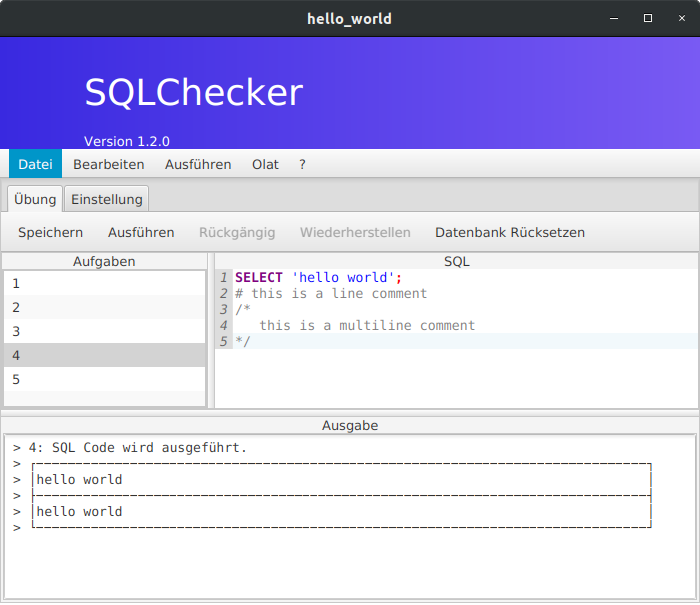
\includegraphics[width=1.0\textwidth]{figures/main}
\smallskip
Das Hauptfenster besteht aus folgenden Bereichen:
\begin{itemize}
	\item[\ref{subsec:Toolbar}.] Die Toolbar	
	\item[\ref{subsec:Uebung}.] Der Übungsreiter
	\item[\ref{subsec:Einstellung}.] Der Einstellungsreiter
	\item[\ref{subsec:Ausgabe}.] Die Ausgabe
\end{itemize}
\subsection{Die Toolbar}
\label{subsec:Toolbar}

\includegraphics[width=1.0\textwidth]{figures/toolbar}
Die Toolbar besteht aus diesen Menüpunkten:

\begin{itemize}
	\item[\ref{subsubsec:Datei}.] Datei
%		\begin{itemize}
%			\item[\ref{item:Neu}.] Neu ...	
%			\item[\ref{item:Oeffnen}.] öffnen ...
%			\item[\ref{item:Speichern}.] Speichern
%			\item[\ref{item:SpeichernUnter}.] Speichern Unter ...
%			\item[\ref{item:LadeKonf}.] Lade Konfigurationsdatei ...
%			\item[\ref{item:ExportKonf}.] Exportiere Konfigurationsdatei ...
%			\item[\ref{item:close}.] Schließen
%		\end{itemize}
	\item[\ref{subsubsec:Bearbeiten}.] Bearbeiten
%		\begin{itemize}
%			\item[\ref{item:undo}.] Rückgängig
%			\item[\ref{item:redo}.] Wiederherstellen
%		\end{itemize}
	\item[\ref{subsubsec:run}.] Ausführen
%		\begin{itemize}
%			\item[\ref{item:reset}] Datenbank Rücksetzen
%			\item[\ref{item:runTask}] Aufgabe Ausführen
%			\item[\ref{item:runComplete}] Vollständig Ausführen
%		\end{itemize}
\item[\ref{subsubsec:Abgabe}.] Abgabe
%		\begin{itemize}
%			\item[\ref{item:export}] Exportieren ...
%		\end{itemize}
	\item[\ref{subsubsec:?}.] ?
%		\begin{itemize}
%			\item[\ref{item:about}] Über
%		\end{itemize}
\end{itemize}
\subsubsection{Datei}
\label{subsubsec:Datei}
Im Menüpunkt Datei finden sich folgende Funktionen:
\begin{description}
	\item[\label{item:Neu}Neu ...] Erstellen Sie ein neues Projekt. Sie werden zunächst aufgefordert eine Aufgaben-Template-Datei auszuwählen. Die Template-Dateien enden auf *.sqlt und werden mit den Übungsaufgaben mitgeliefert.
	
	Wählen Sie nun den Ort für Ihr Projekt. Die Projekt-Datei endet auf *.sqlc.
	\item[\label{item:Oeffnen}Öffnen ...]
	Öffnen Sie ein vorhandenes Projekt. Projekt-Dateien enden auf *.sqlc.
	\item[\label{item:Speichern}Speichern] Speichern Sie das aktuelle Projekt am ausgewählten Projekt-Pfad.
	\item[\label{item:SpeichernUnter} Speichern Unter ...] Wählen sie einen neuen Projekt-Ort. Die Projekt-Datei endet auf *.sqlc. Das Projekt am alten Ort bleibt bestehen.
	\item[\label{item:LadeKonf}Lade Konfigurationsdatei ...]
	Wählen Sie eine Konfigurationsdatei. Konfigurationsdateien enden auf *.conf. Die Konfigurationsdatei wird geladen und die aktuelle Konfiguration wird überschrieben.
	\item[\label{item:ExportKonf}Exportiere Konfigurationsdatei ...]
	Exportieren Sie die aktuelle Konfiguration, um sie für ein anderes Projekt wieder zu verwenden. Wählen Sie den gewünschten Ort. Konfigurationsdateien enden auf *.conf.
	\item[\label{item:close}Schließen] Schließen Sie das aktuelle Projekt.
\end{description} 

\subsubsection{Bearbeiten}
\label{subsubsec:Bearbeiten}
\begin{description}
	\item[\label{item:undo} Rückgängig] Die letzte ausgeführte Veränderung im aktiven SQL-Feld wird widerrufen.
	\item[\label{item:redo} Wiederherstellen] Die letzte rückgesetzte Veränderung im aktiven SQL-Feld wird wiederhergestellt.
\end{description}

\subsubsection{Ausführen}
\label{subsubsec:run}
Um die folgenden Punkte ausführen zu können, müssen die Datenbank-\linebreak Informationen \ref{subsubsec:Datenbank} richtig gesetzt worden sein und MySQL oder MariaDB müssen laufen.
\begin{description}
	\item[\label{item:reset} Datenbank Rücksetzen] Das Reset-Skript wird ausgeführt. Bei fehlerlosen Durchlauf ist die Datenbank wieder im Initial-Zustand. Im Ausgabe-Feld erhalten Sie weitere Information zum Status des Rücksetzens. 
	\item[\label{item:runTask} Aufgabe ausführen] Das SQL-Statement der aktiven Aufgabe wird ausgeführt. Das Ergebnis wird im Ausgabe-Feld angezeigt.
	\item[\label{item:runComplete} Vollständig Ausführen] Die SQL-Statements aller Aufgaben werden nacheinander ausgeführt. Dies ist sinnvoll, wenn die Aufgaben voneinander abhängig sind.
\end{description}

\subsubsection{Abgabe}
\label{subsubsec:Abgabe}
\begin{description}
\item[\label{item:export} Exportieren ...] Erstellen Sie die Abgabe-Datei am gewünschten Ort. Laden Sie diese in ihren Online-Kurs unverändert hoch.
\end{description}

\subsubsection{?}
\label{subsubsec:?}
\begin{description}
	\item[\label{item:about} Über] Zeige das Über-Fenster an.
\end{description}

\subsection{Übung}
\label{subsec:Uebung}
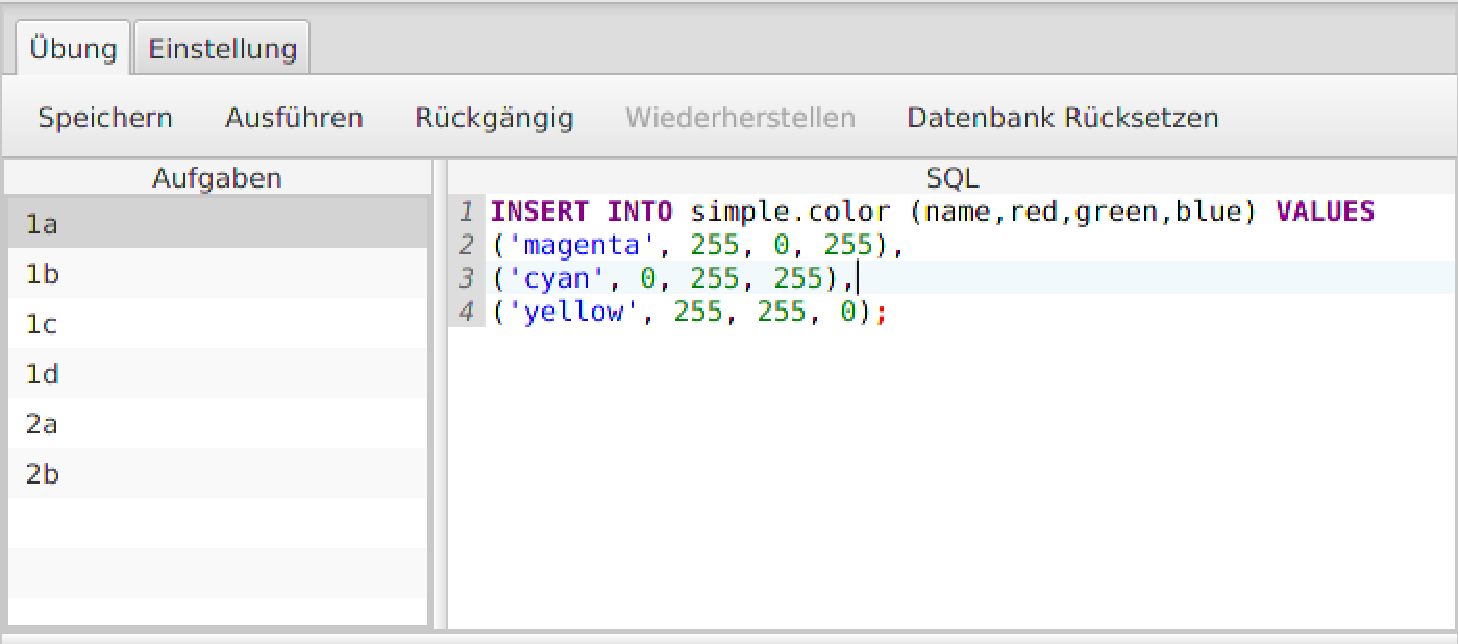
\includegraphics[width=1.0\textwidth]{figures/exercise}
Hier werden die Lösungen der Aufgaben erstellt. Auf der linken Seite sehen Sie die Liste aller zu bearbeitenden Aufgaben \ref{subsubsec:Aufgaben}. Auf der rechten Seite werden die zu erstellenden SQL-Statements im SQL-Feld \ref{subsubsec:SQL} eingetragen. Am oberen Rand des Reiters sehen sie eine Reihe von Menüpunkten \ref{subsubsec:AufgabenMenu}.

\subsubsection{Aufgaben}
\label{subsubsec:Aufgaben}
In diesem Feld steht eine Liste aller Aufgaben. Klicken Sie die Aufgabe an, die Sie bearbeiten wollen. Die Lösung zu dieser Aufgabe tragen Sie im SQL-Feld ein. Sie sollten die Aufgaben von oben nach unten bearbeiten, da tiefere Aufgaben von früheren Aufgaben abhängig sein können.   

\subsubsection{SQL}
\label{subsubsec:SQL}	
Tragen Sie hier die Lösung für die im Aufgaben-Feld ausgewählte Aufgabe ein. Eine Lösung besteht in der Regel aus \underline{einem} SQL-Statement. Sollten weitere erwünscht sein, wird dies explizit gefordert. Wird mehr als ein SQL-Statement eingetragen, obwohl nicht gefordert, wird die Aufgabe mit Null Punkten bewertet.

\subsubsection{Menüleiste}
\label{subsubsec:AufgabenMenu}
\begin{description}
	\item[Speichern] Siehe \ref{item:Speichern}.
	\item[Ausführen] Siehe \ref{item:runTask}.
	\item[Rückgängig] Siehe \ref{item:undo}.
	\item[Wiederherstellen] Siehe \ref{item:redo}.
	\item[Datenbank Rücksetzen] Siehe \ref{item:reset}.
\end{description}

\subsection{Einstellung}
\label{subsec:Einstellung}
Der Reiter Einstellung besteht aus den beiden Punkten Datenbank und Student.

\subsubsection{Datenbank}
\label{subsubsec:Datenbank}
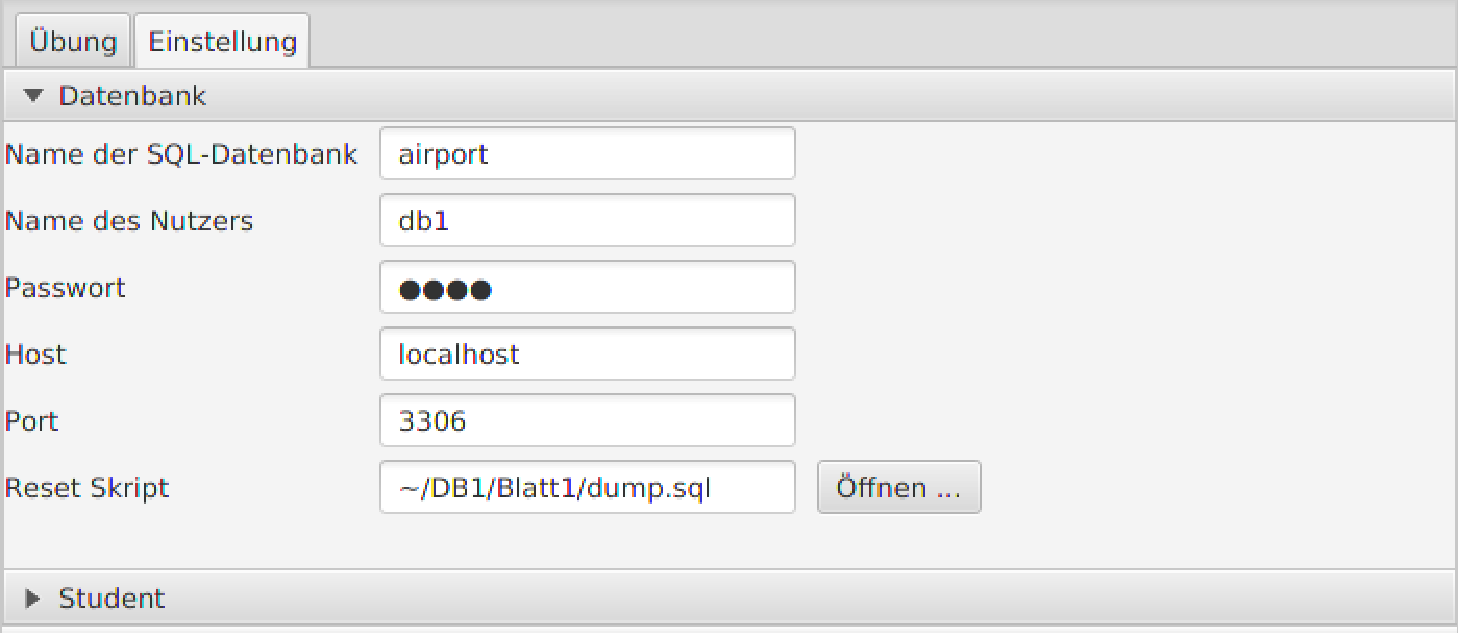
\includegraphics[width=1.0\textwidth]{figures/db}
Tragen Sie hier die Datenbank-Informationen ein. Achten Sie bitte darauf, dass der Nutzer angelegt wurde, das Passwort stimmt und der Nutzer über die nötigen Rechte der Datenbank verfügt.

\begin{description}
	\item[Name der SQL-Datenbank] Der Name der Datenbank auf der die SQL-Statementes ausgeführt werden soll. Nachträgliches wechseln der aktiven Datenbank mittels \fbox{USE \textit{name};} ist nicht möglich. Stellen Sie sicher, dass diese in Ihrer Datenbank existiert.
	\item[Name des Nutzers] Der Nutzername für die Datenbankverbindung.
	\item[Passwort] Das Passwort des Nutzers.
	\item[Host] Der Host des Datenbank-Servers. Wird die Datenbank auf Ihrem Rechner ausgeführt, belassen Sie den Eintrag auf localhost.
	\item[Port] Der Port der Datenbank. Der Standardwert ist 3306.
	\item[Reset Skript] Der Pfad zum Reset-Skript. Das Reset-Skript besteht aus einer Reihe von SQL-Befehlen, welche die Datenbank wieder in den für die Aufgabe vorgesehenen Initial-Zustand bringt. Eine Reset-Skript-Datei endet auf *.sql.
\end{description}

\subsubsection{Student}
\label{subsubsec:Student}
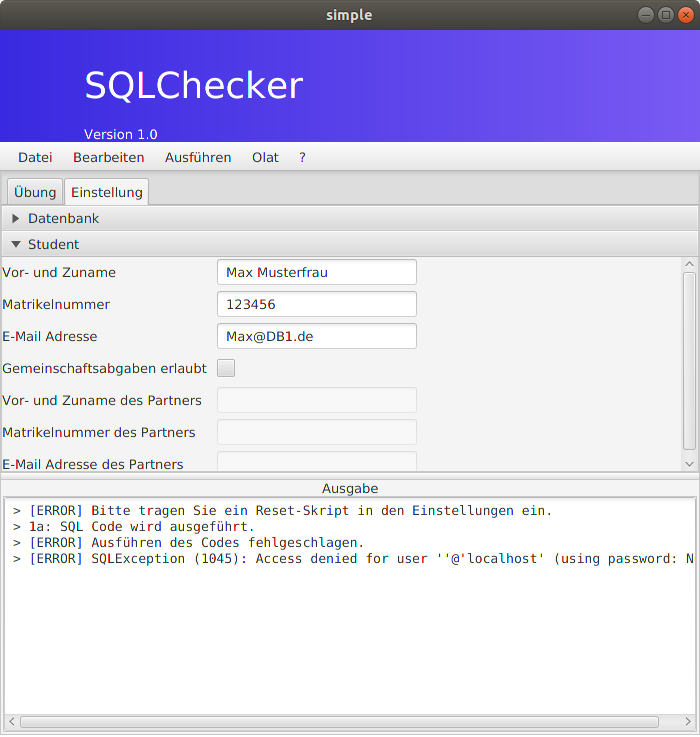
\includegraphics[width=1.0\textwidth]{figures/student}
Hier werden die Information zu den Autoren der Abgabe eingetragen. Die Angaben sind für die Abgabe zwingend erforderlich. Ohne diese Einträge wird die Abgabe mit \underline{Null} Punkten bewertet.

\begin{description}
	\item[Vor- und Zuname] Tragen Sie hier Ihren Namen ein.
	\item[Matrikelnummer] Hier wird Ihre Matrikelnummer erwartet.
	\item[E-Mail Adresse] Der Ort für Ihre E-Mail Adresse.
	\item[Gemeinschaftsabgaben erlaubt] Setzen Sie den Haken, wenn Ihnen gestattet wurde Abgaben mit einem Partner zu bearbeiten. Vergessen Sie nicht die Angaben für Ihren Partner.
\end{description}

\subsection{Ausgabe}
\label{subsec:Ausgabe}
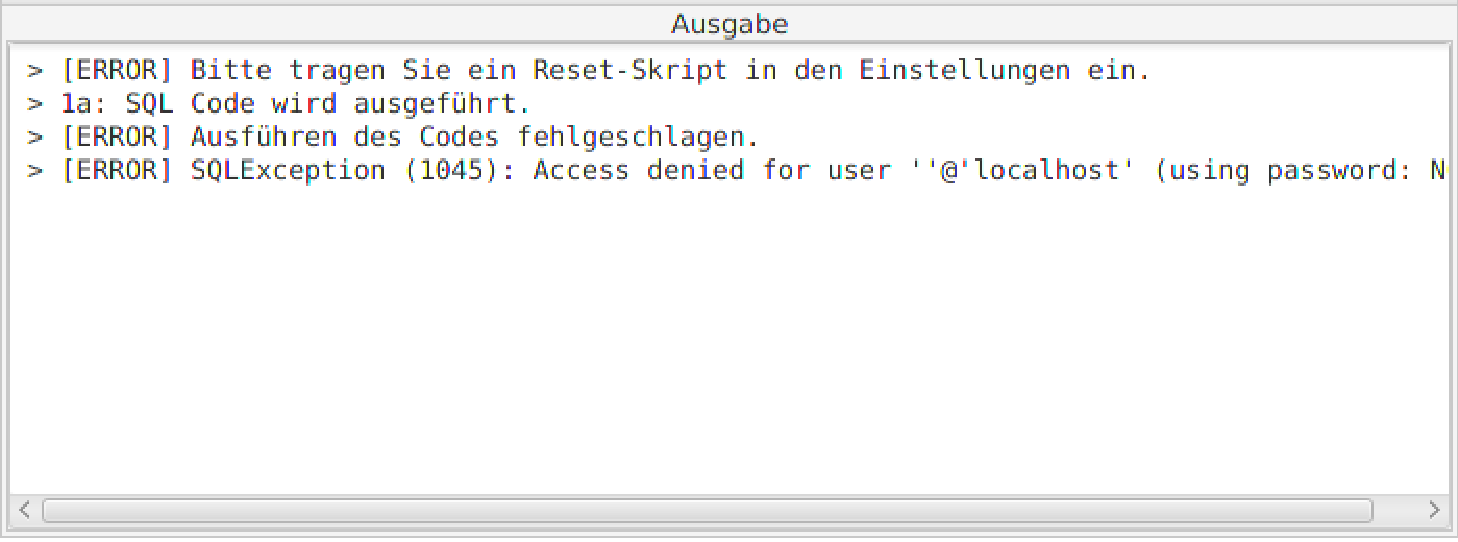
\includegraphics[width=1.0\textwidth]{figures/out}
Hier werden alle produzierten Informationen ausgegeben. Insbesondere sind dies Informationen von der Datenbank und Ergebnisse nachdem Sie ein SQL-Statement ausgeführt haben.

Sie können die aktuelle Ausgabe löschen, indem Sie \fbox{Rechtsklick - löschen} ausführen.

\end{document}
